% !TEX TS-program = pdflatex
% !TEX encoding = UTF-8 Unicode
\documentclass[12pt]{report}
\usepackage[utf8]{inputenc} % set input encoding (not needed with XeLaTeX)

\usepackage{geometry} % to change the page dimensions
\geometry{a4paper} % or letterpaper (US) or a5paper or....
\geometry{margin=2cm} % for example, change the margins to 2 inches all round

% Packages
\usepackage{pdflscape}
\usepackage{graphicx} % support the \includegraphics command and options
\usepackage[parfill]{parskip} % Activate to begin paragraphs with an empty line rather than an indent
\usepackage{booktabs} % for much better looking tables
%\usepackage{array} % for better arrays (eg matrices) in maths
%\usepackage{paralist} % very flexible & customisable lists (eg. enumerate/itemize, etc.)
%\usepackage{verbatim} % adds environment for commenting out blocks of text & for better verbatim
\usepackage{subfig} % make it possible to include more than one captioned figure/table in a single float
\usepackage{amssymb}
\usepackage{epstopdf}
\usepackage{hyperref}
\usepackage{float}
\usepackage{caption}
\usepackage[table]{xcolor}
\captionsetup[table]{skip=10pt}
\usepackage{url}
\usepackage{wrapfig}
\usepackage{amsmath}
\usepackage{algorithmic}
\usepackage{algorithm}

\usepackage{listings}
\usepackage{color}

\definecolor{dkgreen}{rgb}{0,0.6,0}
\definecolor{gray}{rgb}{0.5,0.5,0.5}
\definecolor{mauve}{rgb}{0.58,0,0.82}

\lstset{frame=tb,
  language=Python,
  aboveskip=5mm,
  belowskip=3mm,
  showstringspaces=false,
  columns=flexible,
  basicstyle={\small\ttfamily},
  numbers=left,
  numberstyle=\tiny\color{gray},
  keywordstyle=\color{red},
  commentstyle=\color{dkgreen},
  stringstyle=\color{mauve},
  breaklines=true,
  breakatwhitespace=true,
  tabsize=2
}

% Headers and Footers
\usepackage{fancyhdr} % This should be set AFTER setting up the page geometry
\pagestyle{fancy} % options: empty , plain , fancy
\renewcommand{\headrulewidth}{0pt} % customise the layout of headers and footers
\lhead{Final Report}\chead{}\rhead{Iain Johnston}
\lfoot{}\cfoot{\thepage}\rfoot{}

% Section Title Appearance
\usepackage{titlesec}
\titleformat{\section}{\large\bfseries}{\thesection}{1em}{\hrule}

% ToC appearance
\usepackage[nottoc,notlof,notlot]{tocbibind} % Put the bibliography in the ToC
\usepackage[titles,subfigure]{tocloft} % Alter the style of the Table of Contents
\renewcommand{\cftsecfont}{\rmfamily\mdseries\upshape}
\renewcommand{\cftsecpagefont}{\rmfamily\mdseries\upshape} % No bold!


% The document content starts below

\title{\textit{Final Report}\\\textbf{Maximising entertainment value in the vote-reveal problem}\\ Final Year Project (CM3203) - 40 Credits}
\author{Author: Iain Johnston (1312579) \\ Supervisor: Richard Booth\\ Moderator: Xianfang Sun}
\date{} % Activate to display a given date or no date (if empty),  otherwise the current date is printed

\begin{document}
\maketitle
\clearpage

\section*{Abstract}

\section*{Acknowledgements}

\tableofcontents %  place a table of contents after the title
\listoffigures
\listoftables
\clearpage % clear the page after the table of contents

%\addcontentsline{toc}{section}{Section z} % how to add an entry to the table of contents that is un-numbered
%\section*{Second Section} % an un-numbered section in the document
%\subsection{A subsection} % an example subsection
\section{Introduction}\label{Introduction}
% tell the reader what the project is about without assuming special knowledge and without introducing any specific material that might obscure the overview.
% anticipate and combine main points described in more detail in the rest
% include things such as:
% the aim(s) or goal(s) of the project,
% the intended audience or “beneficiaries” of the work done,
% the scope of the project,
% the approach used in carrying out the project,
% assumptions on which the work is based and
% a broad summary of important outcomes.
In many elections or competitions, a set of voters will rank a set of candidates from best to worst, or will give scores to some of the candidates, with the winner then being the candidate that gets the highest total number of points. When it comes to revealing the result after all votes have been cast, some competitions proceed by having a roll-call of all the voters in which each announces their own scores. This is often done for entertainment purposes such as in the Eurovision Song Contest.\cite{EurovisionVoting}

The concept of \textit{entertainment}, especially with respect to competition, is a heavily subjective matter and as such is difficult to quantify in simple terms. There are intuitive constituent parts to an \textit{entertaining} competition (like Eurovision) such as, if the winner is known early or late, and how many teams are in the running to win. This project will find ways to translate these slightly nebulous concepts into more concrete mathematical functions.  

The two main questions that this project will aim to answer are:

\begin{enumerate}
\item How can we define the concept of ''entertainment'' in the context of an optimisation problem, and hence try to maximise it.
\item  In which order should the votes be revealed in order to maximise that entertainment value?
\end{enumerate}

To try and answer these questions the Eurovision Song Contest will be used as an example as it has good quality datasets. Furthermore voting rules have gone through changes over the years as more countries joined and as it grew in popularity, giving the project a natural comparison tools throughout. Most recently since the 2016 running of the contest. The scoring rules of Eurovision are also well documented and relatively simple (see \ref{Background} for deeper explanation).

These changes to the voting rules show that the motivation behind this project, to maximise entertainment when revealing the votes, is a current problem and there have been attempts to try and solve this problem already.

There is no specific intended audience of this project, Eurovision is a test competition as it fits well with the more general optimisation problem that this project is trying to solve. In this regard it could be said that the beneficiaries of the project would be those who would also attempt to solve this problem, for other datasets or competitions. This project can help set out a framework for approaching these problems and many parts could even be re-used as long as the problem can be formulated in a specific way (see \ref{Implementation} for details on how)

The scope of this project is to try and solve the problem by finding a globally optimum solution, or by find the best solution possible and hence have a voting order that is the most entertaining. Also within scope is producing a way of visualising the solutions found and from this gaining better insight into why they are entertaining. This project does not try and influence other parts of the voting that could also lead to more entertainment (such as who delivers the votes or other human traits, only the order itself)

The approach to tackle this problem is a scientifically minded one. There are three main sections to the project. Firstly, designing and implementing functions that quantify the entertainment of a given voting order. Secondly, solving the optimisation problem of maximising the entertainment value given by those functions; using optimisation algorithms. Finally, analysing the solutions given and comparing and contrasting why there are entertaining and how well the algorithms did in finding them. This approach involves iteration on theoretical ideas whilst feeding back in results as the project goes along.

The important outcomes of this project are, a solution that delivers an entertaining competition when the votes are revealed, a way of describing entertainment mathematically, and a way of visualising the competition as the votes are revealed.

\section{Background}\label{Background}
% give reader info that they can't be expected to know, but which they need in order to fully understand and appreciate the report
% explain why the project is addressing the problem described in the report
% indicate an awareness of other relevant work
% show clearly that the problem has not been solved by anyone else
% include things such as:
% the wider context of the project,
% the problem that has been identified,
% likely stakeholders within the problem area,
% any theory associated with the problem area,
% any constraints on the approach to be adopted,
% existing solutions relevant to the problem area, and why these are unsuitable or insufficient in this particular case,
% methods and tools that your solution may be based on or use to solve the problem,
% you should also refer to the general problem for which these algorithms are useful (the application(s) for your techniques).
% existing products, documents or artefacts that you should mention could be:
% similar to the one you are proposing,
% support your project,
% your project aims to extend or replace,
% demonstrate the “deficiencies” your project intends to address.
The more general reason for this project is to try and see if there can easily be found an optimal solution to a problem when given a mathematical representation of something that humans experience. 

Moreover in competitions where voting is revealed, such as in Eurovision, one of the only ways to change how entertaining the competition seems, is to change the order. Any other changes to the actual running of the competition are unethical.

Furthermore as competitions are usually televised or watched live, it is generally in the interest of those in charge of the competition to produce an entertaining show as this helps them with many facets of their business such as through advertising, but also in building a following for the competition. In this way, it is obvious that a more exciting competition leads to more engaged fans.

\subsection{Project Context}\label{Project Context}
Eurovision has been a topic of research for many years now. The main focus of that research has been in relation to the voting patterns that can be found over the course of many runnings of the competition. This research such as \textit{"Comparison of Eurovision Song Contest Simulation with Actual Results Reveals Shifting Patterns of Collusive Voting Alliances"}\cite{gatherer2006}, \textit{"Geography, culture, and religion: Explaining the bias in Eurovision song contest voting"}\cite{so66198} and \textit{"The Eurovision Song Contest. Is voting political or cultural?"} \cite{Ginsburgh200841} all use the Eurovision Song Contest as a basis to investigate political and cultural phenomena.

There have also been some more computational view of Eurovision such as \textit{"Using the Clustering Coefficient to Guide a Genetic-Based Communities Finding Algorithm"}\cite{Bello2011} which attempts to find communities within the voting patterns.

The particular problem this project is addressing has not been approached in a scientific setting as yet. It does seem to have been at least tackled by those that run Eurovision however not with exactly the same data and considerations. Moreover as they are a private company they have never published any methodology on how they pick voting orders. They usually state on their website when revealing the voting order that 
\begin{verbatim}"The voting order has been determined by the results from last night's Jury Final.
An algorithm has been created to try and make the voting as exciting as possible."
\end{verbatim}\cite{votingOrderQuote}
There is no mention of how this algorithm works or what they constitute entertaining or exciting.

The biggest drawback that can be said about the current Eurovision algorithm, without seeing it and understanding its methodology, is that it only takes into account Jury votes as they can be decided on during the dress rehearsals. This is problematic as the Jury and tele-voting can diverge for many reasons and hence the voting order that purports to be entertaining, may only be such when the viewers at home agree exactly with the Jury.

This project's method takes into account both the sets of votes and hence could give a more correct picture of what will happen, entertainment wise, for any given voting order. One main deficiency with this method is that fact, as it is necessary to wait for all the votes to be cast and then the voting order can be found. In real world terms this may not be feasible for the Eurovision Song Contest as they may have commitments that require that the voting order is known in advance for various logistical reasons.

Another drawback as mentioned above, is the fact that there is no explanation as to why their algorithm believes a given order to be more exciting than any other. This project will attempt to standardise mathematically a function for entertainment, which could in future be compared through human tests (see \ref{FutureWork}).By describing a concept mathematically not only can it be used by algorithms but it can also form part of a proof of which a general thought put forward by a human cannot be.

This project only looks at one specific area of the competition to describe and codify entertainment. This can be seen as a drawback of the solutions found, however the way this project has been undertaken leaves the opportunity of further work in the area of defining entertainment functions as described in \ref{FutureWork}.

The techniques used and implemented in this project have applications outside the strict problem that is being solved here. For example even though this problem is specifically trying to produce entertaining orders for Eurovision, there is no reason why other competitions who use the same type of ordered voting system (sometimes referred to as roll-call voting) could use the algorithms and framework designed and implemented in this project to solve their problems. 

\subsection{Background Theory}\label{BackgroundTheory}
Understanding how the Eurovision Song Contest voting works is key to this project, as this affects many parts of the design and implementation of entertainment functions. Furthermore the system for voting has been changed over many years and so to try and standardise the project I will be using the system that was in use during the 2014 running of the competition, and the main dataset also comes from that year.\footnote{2014 voting system is the system that had been in use from 2009 and changed in 2016}

In this system, each country awards two sets of 12, 10, 8–1 points to their 10 favourite songs: one from their professional jury and the other from tele-voting. Moreover as voting is done by both and jury and by people voting by phone, both constituent parts count 50\% towards the final score.

In the 2014 contest, there were 37 countries that participated and of those 26 reached the final. All 37 countries vote in the final. From this point on in this report, the countries that vote are referred to as \textit{voters} and those 26 competing in the final are referred to as \textit{participants}. There is overlap between the two groups i.e the \textit{participants} set is a subset of the \textit{voters} set; but it should be obvious from the context to whom is being referred.

\begin{figure}[H]
\centering
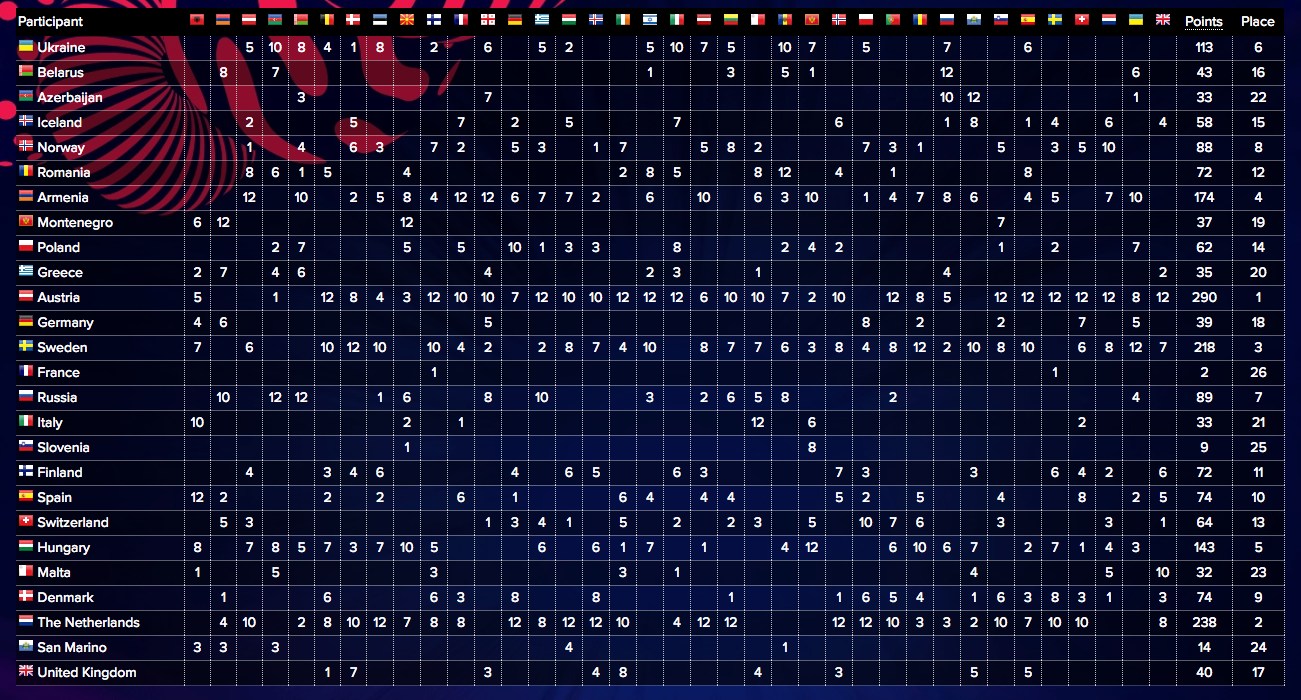
\includegraphics[width=15cm, height=7cm]{./2014Scoreboard}
\caption{2014 Scoreboard}
\label{f_2014Scores}
\end{figure}

This voting system creates a matrix of scores as seen in Figure \ref{f_2014Scores}. The \textit{voters} are arranged along the top alphabetically, while the \textit{participants} are along the left hand side. Points refers to the final total of all the scores given at the end of all voting, and rank is their final position in the competition. 

This is important to look at as it can help clarify what this project's aim is. A solution to the problem is found by moving the \textit{voters} along the top into different positions and then analysing the scores after each country has voted, to reach an \textit{entertaining} order for those countries to reveal their votes.

% Your background section should end with a clear statement of the research questions problem your project is trying to answer. 
%These will reflect the aim of your project, but will be different in that they explain the problem you are attempting to solve
Hence the problem that this project is trying to solve is about ordering who votes when so as to maximise some mathematical concept of entertainment. Should the order put Spain and France next to each other in the order, or would it be better if they were split up. Should Ukraine's vote be near the start or near the end so that the competition is exciting. This is what the project is trying to decide.

\section{Algorithm Designs/Approach}\label{AlgorithmDesigns}
% give reader a clear picture of the system
% specification becomes: description of the problem and what is required of a solution
% design becomes: description of your approach to solving the problem and your suggested solution(s)
% problem statement section and then a section describing one or more suggested algorithms to solve the problem
% Later in results and evaluations describe how to design experiments to test how well the algorithms solve the problem and present experimental results with an evaluation of your suggested solutions
% big-O
% reasoning behind writing each algorithm
This section should give an understanding of the main computational parts that are needed to solve this problem, before implementation can be explained. This will include some pseudocode of the algorithms used, explanations of the neighbourhoods tried and the entertainment functions designed. It is intended to give an introduction to the why and how these parts of the project exists, before Section \ref{Implementation} goes into implementation details with code and explanations using Python.

Firstly to help clarify the problem it is easier to view a much smaller competition and then run through the main points of theory, that then are used in the full Eurovision system.

Firstly we design a competition that involves 3 teams total, of which 2 are \textit{participants}. The scoring system is even more simple than the one used by Eurovision. Here each voting team gives 1 point the team they prefer and 0 to the other. A team cannot give itself 1 point. This produces a lot of scores similar to the one in Figure \ref{f_2014Scores}. It is shown in Table \ref{t_simpleMatrix}.

\begin{table}[H]
\centering
\caption{Scores for simple example game}
\label{t_simpleMatrix}
\begin{tabular}{@{}|l|l|l|l|@{}}
\toprule
        & Austria & Spain & France \\ \midrule
Austria & 0       & 1     & 1      \\ \midrule
France  & 1       & 0     & 0      \\ \bottomrule
\end{tabular}
\end{table}

From Table \ref{t_simpleMatrix} we can see how the scores will be calculated in this type of competition. For simplicity, the order that the teams vote is the order from left to right in Table \ref{t_simpleMatrix}. This means that after Austria has voted the scores are $Austria: 0, France: 1$, the rest of the competition is shown in Table \ref{t_simpleScores}

\begin{table}[H]
\centering
\caption{Scores per round}
\label{t_simpleScores}
\begin{tabular}{@{}|l|l|l|l|@{}}
\toprule
        & After Austria's vote & After Spain & After France \\ \midrule
Austria & 0       & 1     & 2      \\ \midrule
France  & 1       & 1     & 1      \\ \bottomrule
\end{tabular}
\end{table}

We can see that France wins this competition, with 2 points. This cumulative scoring extends to the full Eurovision competition in the exact same way, except for in that case there are 30+ voters.

All that is needed to turn this simple example into Eurovision is to add all the \textit{voters} and \textit{participants} and change the scores given out to be $12, 10, 8-1$ instead of just 1 and 0.

\subsection{Entertainment Functions}\label{EntertainmentFunction}
From the small example, it is quite easy to think of some theoretical reasons why a given order is entertaining. This leads straight into the design of entertainment functions and how they model entertainment. 

It is important to start with the design of the entertainment functions as they are the main workhorse part of finding solutions to the problem. The approach was to analyse the competition and try and identify things in a competition that lead to excitement. From those ideas, it was a case of trying to formalise that theory into a concrete piece of maths that could then be programmed. Furthermore the entertainment functions are quite problem specific and may not transfer well into other problems, whereas the algorithms are entirely agnostic to the problem at hand. This means the entertainment functions follow much more closely from the problem itself than any other part of the project.

Any entertainment functions talked about in this section share some characteristics that need to be explained. The first is that they take a \textbf{solution ($\Phi$)} to the problem (see Glossary-3) as input and they return a single \textbf{entertainment value} ($\varepsilon$) (see Glossary-4). Moreover they calculate the \textbf{scores}($S$) (see Glossary-6) for each \textit{participant} country every \textbf{round} ($R$)(see Glossary-5).

\subsubsection{MaxMin}
The first entertainment function that was designed is named \textbf{MaxMin} and as it's name suggests it works by finding the difference between the highest score (max) and the lowest score (min) after each voting round. It then sums the value which is the $\varepsilon$ value for that solution. This function follows quite naturally from watching and analysing the Eurovision competition as the way roll-call style voting works, everything is building towards the later end of the voting order. Hence it seems to be a innate part of the competition that you would want every country to be in with a chance of winning for as many rounds as possible. Moreover as there is only one prize, for first place, it is even less important to worry about positioning other than the top.

So each round the distance ($\Lambda$) is calculated as such:
\begin{equation}\label{lambda}
	\Lambda = \max(S) - \min(S)
\end{equation}

Then keeping the distance per round $i$ as $\Lambda_i$, the entertainment value ($\varepsilon$) is found by:
\begin{equation}\label{epsilon}
	\varepsilon = \sum_{i=0}^{n_R}  \Lambda_i
\end{equation}

This is a relatively simple equation and hence transfers simply to code. However more importantly, it encodes an intuitive part of entertainment mathematically. These functions encode the fact that an entertaining competition is one in which the distance between first and last place is as low as possible as often as possible. In this case instead of maximising $\varepsilon$, we want to minimise it.

Over the course of a whole competition i.e: $n_R$ voting rounds, it is intuitive to want that distance to stay as low as possible. Hence finding the sum of the distance ($\Lambda$) in each round and then using optimisation algorithms to try and find a solution ($\Phi$) that minimises this value.

However there is one major drawback of the basic MaxMin method, which is that in some rounds, especially later in the competition, the last place country is actually mathematically eliminated from the race for first place.

\subsubsection{RefinedMaxMin}
This leads to a second version of the entertainment function for this problem. As it is essentially a refinement of the first function and not a brand new method it is called \textbf{RefinedMaxMin}.

Equation \ref{epsilon} is the same across both functions, however where \textbf{RefinedMaxMin} and \textbf{MaxMin} differ is how the $\min$ part of equation \ref{lambda} is calculated. As some of the countries cannot win the competition after some number of rounds, they should not be taken into account when seeing if a solution is entertaining or not.

To find whether a team can still win, the upper bound of points left available is found. This means that we assume for each team, and for the remaining rounds left to be revealed, that they gain the maximum (12) points and the hence we find the highest score they could ever attain. This method does not take into account whether the country has already given itself a vote (in which case they would not be allowed to get 12 points in that round). This was done to simplify the method and make testing it's improvements against MaxMin easier. Furthermore finding the upper bound is generally safe, especially when removing the low scoring teams in Eurovision as voting is generally quite uniform past a certain point in the voting; i.e countries that are given high points already generally get more, and countries that have received few points continue to get few.

The method for finding if a team can still win is to first sort the scores for every country in round $i$ in ascending order. Then iterating through that list of scores from the start and for each score checking whether equation \ref{stillWin} is true.
\begin{equation}\label{stillWin}
	countriesScore + (maxScorePerRound * roundsRemaining) < currentTopScore
\end{equation}

If equation \ref{stillWin} hold true then that country cannot win even if it received the maximum number of points (12 in Eurovision's case) and the leaders received the worst score possible (0), for the remaining voting rounds. As the scores are in ascending order the last minScore found for which Equation \ref{stillWin} held true is the minimum score to be returned.

It is quite simple to justify this refinement when looking at the competition. Those teams who cannot win should will not be making a mark on the entertainment of the voting order as most viewers will not be paying attention to their scores. Moreover this refinement only works in competitions where there is only interest at the top of the table as opposed to competitions with relegations or play-offs, where more than just who is the overall winner is important.

\subsection{Neighbourhoods}\label{Neighbours}
An important part of solving optimisation problems is designing and implementing neighbourhoods for given solutions. As a solution ($\Phi$) is a list of \textit{voters} in a certain order, then we define a neighbourhood a solution as any other solution that has two members swapped. This means that there are only two changes between a solution and any of it's neighbours.

In this regard an order is a \textit{permutation} of the \textit{voters}. Using Cauchy's two line notation for permutations\cite{Cauchy}, we can show the basic theory for neighbourhoods.

\begin{equation}\label{neighbourhood}
\begin{pmatrix}
x_{1} & x_{2} & x_{3} & \cdots & x_{n} \\
\sigma(x_{1}) & \sigma(x_{2}) & \sigma(x_{3}) & \cdots & \sigma(x_{n}) \\
\end{pmatrix}
\end{equation}

Equation \ref{neighbourhood} shows the first solution on the top row and a neighbour of that solution on the bottom row. The functions that map the elements of a solution to a neighbour ($\sigma$) are explained below.

These methods are examples of cyclic permutations i.e a permutation of a set which maps a subset of elements to each other in a cyclic way, while mapping to themselves all other elements of the set. The cyclic parts of a permutation are called \textit{cycles}. A cycle with only two elements is called a \textit{transposition}\cite{cyclicPerm}. As both the methods following only contains two indexes, they are transpositions.

\subsubsection{Random neighbour}
The first idea and most simple for this problem, was to swap two random elements of the ordering. This means that the function $\sigma$ swaps the two elements at those indexes. This method can be described as such in equation \ref{random}.

\begin{equation}\label{random}
\begin{split}
	\sigma_r = x_i \mapsto x_j,\\ x_j \mapsto x_i,\\ \forall x \neq i \lor \forall x \neq j: x \mapsto x
\end{split}
\end{equation}

for two random indexes $i$ and $j$

This means that we swap the elements at indexes i and j and swap the rest with themselves. The code for this will be explored in Section \ref{Implementation}. This method give a large possible neighbourhood as theoretically for any single solution there are \{length of solution $\times$ length of solution - 1\} possible neighbours. In the 2014 Eurovision competition this would mean $\{37 \times 36 = 1332\}$ neighbours.

This method may be simple however, when a closer look is taken at the $\varepsilon$ values of solutions that are very similar to each other i.e they have 3 or 4 elements swapped, it is clear that their $\varepsilon$ values only differ by a little. This calls into question if the method detailed above is actually going to help the optimisation algorithm reach an optimal solution.

\subsubsection{Adjacent neighbour}
Those questions about the efficacy of the random method leads to another method for finding a neighbour of a solution. As solutions that are close together are usually quite similar, it is intuitive that swapping adjacent elements may improve the performance.

This method works by finding a random value between 0 and length of solution - 1. Then swapping the element at that index with its immediate neighbour to the right i.e. index + 1. It can be expressed in the same way as in equation \ref{random} in equation \ref{adjacent}, except that in this case index $i$ is a random number and index $j = i + 1$.

\begin{equation}\label{adjacent}
\begin{split}
	\sigma_a = x_i \mapsto x_j,\\ x_j \mapsto x_i,\\ \forall x \neq i \lor \forall x \neq j: x \mapsto x
\end{split}
\end{equation}

Another difference between this method and the random method is how it can actually be calculated. After finding a neighbour of a given solution, the $\varepsilon$ value of that solution must be found. By swapping 2 adjacent countries in the solution a \textit{partial re-calculation} of the entertainment value can be done using the entertainment value of the previous solution. 

As the previous solution and the new solution only differ by one position it is possible to only partially re-calculate the $\varepsilon$ value. Re-calculation involves removing the distances for the two rounds of the swapped countries in the old solution and adding them back in their new positions in the new solution. The equation for this is shown in \ref{Recalc}
\begin{equation}\label{Recalc}
	\varepsilon_{new} = \varepsilon_{old} - \Lambda_{ij_{old}} + \Lambda_{ij_{new}}
\end{equation}

The $\varepsilon_{new}$ and $\Lambda_{ij_{old}}$ values can be found by keeping them from the old solution and passing them into the $\varepsilon$ calculation function. The $\Lambda_{ij_{new}}$ must still be re-calculated however only up to the index of the higher of the two indexes.

A deeper comparison and evaluation between the two methods can be found in Section \ref{Results}

\subsection{Optimisation Algorithms}\label{Algorithms}
In the previous section the necessary steps to solve the problem were outlined. Namely calculate an entertainment value ($\varepsilon$) which can be optimised. To do this it is necessary to use a set of optimisation algorithms which maximise or minimise a value in order to settle on an optimal solution.

\subsubsection{Greedy Search}
The first algorithm that was posited was a simple greedy search algorithm. Greedy search works on the idea that by selecting the optimal choice at every possible stage, it will lead to a globally optimal solution. 

At first glance it is not obvious to see if the problem we are attempting is simple or complex. This lead to greedy search as a good first try as it is sufficiently simple to allow for easy writing of the code and will likely find the optimal solution if the solution space is relatively simple. If the solution space \textit{is} in fact too complex then greedy may instead find a good approximation for the problem.

The pseudocode for greedy is shown in Algorithm \ref{greedyCode}

\begin{algorithm}
\caption{Greedy Search}
\label{greedyCode}
\begin{algorithmic}[1]
\REQUIRE list of voters
\REQUIRE scoreBoard
\REQUIRE list of performers
\STATE $xNow \leftarrow getInitialSolution()$
\STATE $xBest \leftarrow getInitialSolution()$
\STATE $entertainmentXBest \leftarrow getEntertainment(xBest)$

\WHILE{$i < maxIterations$}
\STATE $xNow = getNeighbour(xNow)$
\STATE $entertainmentXNow = getEntertainment(xNow)$

\IF{entertainmentXNow $<$ entertainmentXBest}
\STATE $xBest = xNow$
\STATE $entertainmentXBest = entertainmentXNow$
\STATE $i = 0$
\ENDIF
\STATE $i = i + 1$
\ENDWHILE
\RETURN XBest, EntertainmentXBest
\end{algorithmic}
\end{algorithm}

As can be seen, it is a very simple algorithm that takes possible solutions and compares them to the already found best solution. It's simplicity is, unfortunately, also it's downfall in this problem. Although it can find a good approximate solution it is not able to find optimal solutions that other algorithms do find.

Looking at the pseudocode, and with some simplifying assumptions the time complexity for this greedy search implementation can be found.

This is done by giving all the instructions that make a difference to complexity, a value $T_i$ from their line number. This means line 5 is $T_5$, then working out how many times that instruction will need to be run given an input. The input is the \textit{voters} and \textit{participants}, $V$ and $P$. Some lines can be ignored as they do very little to complexity.

Firstly,

$T_1$ = run once with $V$ steps

$T_2$ = run once

$T_3$ = run once with $V \times P$ steps

The main loop (lines 6 - 15) is constant, given it comes from \textit{maxIterations}. It adds $m$ times to the instructions inside it. So:

$T_5 = m$ times with constant steps

$T_6 = m$ times with $V \times P$ steps; as worst case, assume that full re-calculation is needed

$T_7 - T_{11}= m$ times as is worst case, so assume this block always run

$T_{12}= m$

$T_{14} = 1$

Factoring this down into equation \ref{greedyComp} gives: 

\begin{equation}\label{greedyComp}
\begin{aligned}
	f(n) ={} & \ (V \times T_1) + T_2 + (V \cdot P \times T_3) + (m \times T_5) + (m \times V \cdot P \times T_6) \\
	 	& + (m \times T_{7 - 11}) + (m \times T_{12}) + T_{14}
\end{aligned}
\end{equation}

From this we can safely ignore anything that is less than the highest order as it will dominate the complexity growth. Moreover we can see that the highest order is $T_6$, so we are left with equation \ref{greedyCompSimp}

\begin{equation}\label{greedyCompSimp}
\begin{aligned}
	f(n) ={} & \ (m \times V \cdot P \times T_6) \approx m \times V \cdot P
\end{aligned}
\end{equation}

where $P <= V \ll m$. This can be further simplified in terms of \textit{voters} ($V$), as $P$ is always less than or equal to $V$ and $m$ is always larger or equal to $V$, they can be equated to $V$. The coefficients of $m$ and $P$ compared to $V$ don't matter to the complexity, just that they are near the same size. This leaves us with a fair approximation of the complexity in equation \ref{greedyCompFinal}.\footnote{A full table of Big-O complexity for all algorithms can be found in the appendix in table \ref{bigO}}

\begin{equation}\label{greedyCompFinal}
\begin{aligned}
	O(n) \approx{} & \ m \times V \cdot P \approx V \times V \times V \approx V^3
\end{aligned}
\end{equation}

A discussion and comparison with the other algorithms can be found in Section \ref{Results}.

\subsubsection{Brute force}
After running the greedy algorithm and collecting some initial results it became clear that it would be difficult to know by just looking at the problem, what a good $\varepsilon$ value would be. This lead to the discussion about using a brute force algorithm and if it was possible. 

The implementation is extremely simple, even more so than greedy. The reasons why are to do with Python and are explained in Section \ref{Implementation}. Even though the pseudocode and the real code will differ, the pseudocode help understand the algorithm so is shown in Algorithm \ref{bruteForceCode}

\begin{algorithm}
\caption{Brute Force}
\label{bruteForceCode}
\begin{algorithmic}[1]
\REQUIRE list of voters
\REQUIRE scoreBoard
\REQUIRE list of performers
\STATE $xBest \leftarrow getInitialSolution()$
\STATE $entertainmentXBest \leftarrow getEntertainment(xBest)$

\FORALL{$S \in Solutions$}
\STATE $entertainmentXNow = getEntertainment(S)$

\IF{entertainmentXNow $<$ entertainmentXBest}
\STATE $xBest = xNow$
\STATE $entertainmentXBest = entertainmentXNow$
\ENDIF
\ENDFOR
\RETURN XBest, EntertainmentXBest
\end{algorithmic}
\end{algorithm}

When this code was left to run for around 8 hours it could only find one solution better than the initial solution. When some simple calculations are made about the solution space it is clear as to why the brute force method is not ever going to feasible for this problem. 

Searching all solutions ($V!$), is not a simple task. For example in the 2014 running of Eurovision this would be $37!$ which, after approximating the time to look at one single solution, would take about $1.2\times10^{40}$ seconds, which is quite obviously computationally infeasible with the time and resources for this project.

This means that in all cases brute force will run in $V!$ time. Comparison to the other algorithms used can be found in Section \ref{Results}.\footnote{A full table of Big-O complexity for all algorithms can be found in the appendix in table \ref{bigO}}

\subsubsection{Simulated annealing}
These results reveal the fact that this problem is not a simple one at all and hence another, more capable algorithm is needed to find more optimal solutions. 

The pseudocode for Simulate Annealing can be found in Alorithm \ref{simAnnealingCode}. It is quite a lot more complex than either brute force or greedy search, but that is for good reason.

\begin{algorithm}
\caption{Simulated Annealing}
\label{simAnnealingCode}
\begin{algorithmic}[1]
\REQUIRE list of voters
\REQUIRE scoreBoard
\REQUIRE list of performers
\REQUIRE ti: Initial Temperature
\REQUIRE tl: Temperature length
\REQUIRE cr\_coefficient: cooling coefficient
\STATE $xNow \leftarrow getInitialSolution()$
\STATE $entertainmentXNow \leftarrow getEntertainment(xNow)$
\STATE $xBest \leftarrow getInitialSolution()$
\STATE $entertainmentXBest \leftarrow getEntertainment(xBest)$

\WHILE{$i < maxIterations$}
\FOR{$j$ \TO $tl$}
\STATE $xPrime = getNeighbour(xNow)$
\STATE $entertainmentXPrime = getEntertainment(xPrime)$
\STATE $deltaC = entertainmentXPrime - entertainmentXNow$

\IF{deltaC $<=$ 0}
\STATE $xNow = xPrime$
\STATE $entertainmentXNow = entertainmentXPrime$
\ELSE
\STATE$q = $ random int between 0 and 1
\IF{$q < e^{-deltaC/t}$}
\STATE $xNow = xPrime$
\STATE $entertainmentXNow = entertainmentXPrime$
\ENDIF
\ENDIF
\IF{entertainmentXNow $<$ entertainmentXBest}
\STATE $xBest = xNow$
\STATE $entertainmentXBest = entertainmentXNow$
\STATE $i = 0$
\ENDIF
\ENDFOR
\STATE $t = t $$\times$cr\_coefficient
\STATE $i = i + 1$
\ENDWHILE
\RETURN XBest, EntertainmentXBest
\end{algorithmic}
\end{algorithm}

The skeleton of the algorithm is shared with both the previous algorithms; that is, lines 22 - 25 in Algorithm \ref{simAnnealingCode} are the same as lines 5 - 7 in Algorithm \ref{bruteForceCode} (brute force) and lines 
9 -12 in Algorithm \ref{greedyCode} (greedy).

The important part where they differ is how they pick a solution to try. Brute force tries every solution one-by-one by permuting through the possible solutions. Greedy search picks a neighbour of the current solution and sees if that is better than the best it has seen. Where simulated annealing differs is that is also finds a neighbour of the current solution, however where greedy always takes that solution and compares it to the best, Simulated Annealing does two things before that comparison.

Firstly as can be seen on lines 12- 14 of Algorithm \ref{simAnnealingCode}, it checks whether the new solution is better than the current one. If it is better, then it takes that solution for comparison to the best. However, if it is not better there is still a chance Simulated Annealing will take it for comparison. 

In lines 16 - 19, a check is performed that allows worse solutions than the current to be checked against the best. This is usually named an \textit{"Uphill move"}. The reason for accepting a worse solution is because it allows for a more extensive search for the optimal solution. Line 17 is a feature that is designed to prevent the algorithm from becoming stuck at a local minimum that is worse than the global one.\cite{simAnnealing}. Moreover as it varies with the value of $t$, it allows the algorithm to take worse solutions at the start, but not take the worse solution nearer the end, meaning the \textit{"Uphill moves"} occur so that the algorithm does not get stuck in a local optima.

To find an approximation for the worst case Big-O of Simulated Annealing:

$T_1$ = run once with $V$ steps

$T_2$ = run once with $V \times P$ steps

$T_3$ = run once with constant steps

$T_4$ = run once with $V \times P$ steps

The main loop (lines 5 - 28) is constant, given it comes from \textit{maxIterations}. It adds $m$ times to the instructions inside it.

The inside loop (lines 6 - 25) is also constant, given it comes from the temperature length, \textit{tl}. It adds $l$ times to the instructions inside it.

$T_7 = m \times l$ times with constant steps

$T_8 = m \times l$ times with $V \times P$ steps

$T_8 = m \times l$ times with constant steps

$T_{10} - T_{19} = m \times l$ times with constant steps, this if-else block can be treated as one because one of the two will always be run.

$T_{20} - T_{23} = m \times l$ as it is the worst case, the assumption is that this block is always run

$T_{26} = m$ times with constant steps

$T_{27} = m$ times with constant steps

$T_{29}$ = run once

Factoring this down into equation \ref{simAnnComp} gives: 

\begin{equation}\label{simAnnComp}
\begin{aligned}
	f(n) ={} & \ (V \times T_1) + (V \cdot P \times T_2) + T_3  + (m \times V \cdot P \times T_4) \\
	 	& + (m \times l \times T_7) + (m \times l \times V \cdot P  \times T_8) + (m \times l \times T_9) \\
		& + (m \times l \times t_{10 - 19}) \\
		& + (m \times l \times T_{20 - 23}) \\
		& + (m \times T_{26}) + (m \times T_{27}) + T_{29}
\end{aligned}
\end{equation}

From this we can safely ignore anything that is less than the highest order as it will dominate the complexity growth. Moreover we can see that the highest order is $T_8$, so we are left with equation \ref{simAnnCompSimp}

\begin{equation}\label{simAnnCompSimp}
\begin{aligned}
	f(n) ={} & \ (m \times l \times V \cdot P \times T_8) \approx m \times l \times V \cdot P
\end{aligned}
\end{equation}

where $P <= V <= l <= m$. As before this can be further simplified in terms of \textit{voters} ($V$). In this case, there is an extra term with will be greater than or equal to $V$. This leaves us with a fair approximation of the complexity in equation \ref{simCompFinal}.\footnote{A full table of Big-O complexity for all algorithms can be found in the appendix in table \ref{bigO}}

\begin{equation}\label{simCompFinal}
\begin{aligned}
	O(n) \approx{} & \ m \times l \times V \cdot P \approx V \times V \times V \times V \approx V^4
\end{aligned}
\end{equation}

A full comparison between the algorithms and their complexities is undertaken in Section \ref{Results}.


\subsubsection{Piecemeal}
Part way through the project a slightly different approach to building a solution was suggested. The three algorithms discussed above all have a major thing in common, that they move from a \textbf{full} solution to another.

It was suggested that another methodology for finding a solution could be used. This method moves slightly more towards population-based search methods such as Genetic Algorithms, but is actual really a more simplified version of them, that also uses a greedy search algorithm as it's base. 

This method begins with just one \textit{voter} instead of a full solution. This \textit{voter} can be found randomly or just be the first in the list. Then to pick the next \textit{voter} to add to the solution, the algorithm looks at all the available \textit{voters} it could add and it picks the one that gives the lowest overall $\Lambda$ value. The $\Lambda$ value is the distance between the best and worst who can still win, which at the end is summed to get the solution's $\varepsilon$ value.

It does this over and over until it finds a full solution. Where population-based search methods keep track of a \textit{population} of possible solutions, this method named the \textit{piecemeal} method, builds a solution by being doing a greedy search of the available next \textit{voters}.

This method hopes that by picking the best possible next choice this will lead to a good approximation or globally optimal solution. It acts very much like Greedy Search that has been discussed, and the pseudocode supports that, however by working on partial solutions instead of full solutions, the idea is that it will at least approximate a good solution without having the need to check many full solutions, hence increasing performance, especially for large solution problems.

The pseudocode for it is shown in Algorithm \ref{piecemealCode} and the implementation is discussed in more detail in Section \ref{Implementation}.

The main points of interest are that even though lines 7 - 9 look very similar to the three algorithms discussed before, there is a subtle difference. In this algorithm, the value that is being checked against the best is not entertainment ($\varepsilon$) but the distances ($\Lambda$).

Another point of interest is a more academic one. It is how do you choose what voter is put at the start. The two most obvious choices are randomly choosing one, which complicates the code slightly, or picking the first from the given list of voters, making the code simpler. The choices and their effect on the $\varepsilon$ returned is explored more in Section \ref{Results}

\begin{algorithm}
\caption{Piecemeal Search}
\label{piecemealCode}
\begin{algorithmic}[1]
\REQUIRE list of voters
\REQUIRE scoreBoard
\REQUIRE list of performers

\STATE $[solution] \leftarrow chooseFirstVoter()$
\STATE $best \leftarrow chooseFirstVoter()$
\STATE $[distances] \leftarrow 12$

\FOR{$k=0$ \TO length(voters) -1}
\FORALL{$Voter \in possibleNextVoters$}
\STATE calculate $\Lambda$ with that voter as next in solution

\IF{$\Lambda < bestDistance$}
\STATE $bestDistance= \Lambda$
\STATE $best = Voter$
\ENDIF
\ENDFOR
\STATE $[solution] \leftarrow best$
\STATE $[distances] \leftarrow bestDistance$
\ENDFOR
\STATE $entertainmentSolution \leftarrow sum(distances)$
\RETURN solution, entertainmentSolution
\end{algorithmic}
\end{algorithm}

To come to a solution, the algorithm must look at a descending number of possible next solutions from the length of the solution down to 1. In the 2014 Eurovision, this would be 37 choices in the first round, 36 in the second, 35 in the third etc. until all \textit{voters} are accounted for.

The formula in equation \ref{infiniteSeries} describes the series that this algorithm will take.

\begin{equation}\label{infiniteSeries}
	\sum_{k=0}^{n} \frac{n(n+1)}{2}
\end{equation}
which can then be simplified for Big-O notation into equation \ref{bigOPiecemeal}. This is because for looking at the complexity of algorithms it is most interesting to look at the term that does the most to the complexity, so in this algorithms case it is the $n^2$ term.\footnote{A full table of Big-O complexity for all algorithms can be found in the appendix in table \ref{bigO}}

\begin{equation}\label{bigOPiecemeal}
	\frac{n(n+1)}{2} = \frac{n^2 + n}{2} \approx n^2 + n \approx O(n^2)
\end{equation}

Looking at the Big-O complexity in equation \ref{bigOPiecemeal} and comparing it to the others is done it Section \ref{Results}.

\clearpage
\section{Implementation of System}\label{Implementation}
% describes system but does so at finer level of detail, down to code level
% realisation of concepts and ideas developed earlier
% complete source code should be provided separately
% pick out and describe pieces of code which for example:
% are especially critical in operation of system
% are of particular interest
% illustrate a non-standard or innovative way of implementing an algorithm, data structure
% mention unforeseen problems that you encountered when implementing the system like:
% difficulties involving existing software
% lack of suitable supporting framework
% over ambitious project aims
% A seemingly disproportionate amount of project time can be taken up in dealing with such problems. The Implementation section gives you the opportunity to show where that time has gone.
In this section, the main important parts of the projects code will be explored. This will take the theory and pseudocode described in Section \ref{AlgorithmDesigns} and discuss the actual code implemented as part of the project. It will both discuss some specific code as well as a discussion as to why parts of the system were implemented in certain ways. All code referenced in this section can be found in the attached zip file, submitted along with this report.

\subsection{Entertainment Functions wrappers}\label{Imp-Ewrappers}
The $\varepsilon$ functions form one of the most important parts of this project, however for them to be implemented they need some contextual data. The functions described below are larger functions that wrap around and allow the $\varepsilon$ functions to do their work. The $\varepsilon$ functions actually form just the $min(S)$ part of equation \ref{lambda}. 

These wrapper functions share an important part, which is shown in \ref{findScores}.\footnote{Section of code from \textbf{getEntertainment} in \textit{support.py}. Full function can be found in attached source code}

\begin{figure}[H]
\caption{Calculating the cumulative scores per participant}
\label{findScores}
\begin{lstlisting}
for j in range(len(solution)):
  for i in range(len(countries)):
    v = voters.index(solution[j])
    scores[i] = scores[i] + score_board[i][v]
    ...
\end{lstlisting}
\end{figure}

The main point of interest is the two nested \textit{for} loops and specifically lines 3 and 4.

As the distance ($\Lambda$) is found as the difference between max and min scores in each round, it is necessary to go through and cumulatively add the scores given to each \textit{participant} in every round. This is stored in the array $scores$ at the index for that \textit{participant}: $scores[i]$. The $score\_board$ is the matrix of all scores given, as discussed in Section \ref{Background}. 

These lines are interesting to highlight as they are likely the most critical lines in all the system. Every algorithm must use them at some point and all $\varepsilon$ functions will need them to calculate the $\varepsilon$ value.

As the score lookup is done against a matrix of scores, it is necessary to find the correct column to look in. The row is the current \textit{participant}: $i$, however finding the column is a little more complex. 

The columns in the matrix are in a certain order, normally alphabetical in Eurovision datasets. This, along with the fact that each solution is a permutation of that order, means that the currently voting country in the solution, $solution[j]$, must be found in the original order to correctly retrieve the score it gives. By keeping track of the original order as it corresponds to the scoreboard, the system only ever has to keep one matrix in memory, along with 2 list of \textit{voters} and \textit{participants}. Any other method would include shuffling the scoreboard into the order of the current solution. As the scoreboard grows i.e in other, larger, problems, this method would become untenable and possibly begin adversely affecting the algorithm's runtimes and complexities.

The method $array.index(element)$ returns the index in $array$ of the given $element$. In this case $solution[j]$, would be a country name such as "Germany", and the value of $v$ will be an integer corresponding to the column.

Looking at the full code listings there are actually two methods that wrap around $\varepsilon$ calculation functions to provide them with context and data. These are called \textbf{offsetGetEntertainment} and \textbf{getEntertainment}, and they both share the code shown in Figure \ref{findScores}. They are also fully independent of the \textit{maxMin} and \textit{refinedMaxMin} functions which are the actual $\varepsilon$ functions. These methods differ because of when and why they can be used.

The main reason for these differences is shown in Section \ref{Neighbours} as using different neighbourhood methods leads to different ways to calculate the entertainment. 

\subsubsection{offsetGetEntertainment}
Firstly the more complex \textbf{offsetGetEntertainment} is used in conjunction with adjacent neighbour swaps as it relies on using the previous $\varepsilon$ value. The theory behind why this works is explained in Section \ref{Neighbours}, specifically the Adjacent neighbours subsection and equations \ref{adjacent} and \ref{Recalc}.

This function is shown in Figure \ref{getEntertainment}

\begin{figure}[H]
\caption{getEntertainment method}
\label{offsetGetEntertainment}
\begin{lstlisting}
def offsetGetEntertainment(solution, countries, score_board, voters, key1, oldEntertainment, oldDistances, maxScorePerRound):
    
    entertainmentValue = 0
    performing_countries = countries[:]
    current_solution = solution[:]
    distances = oldDistances[:]
    key2 = key1 + 1

    oldDistance1, oldDistance2 = oldDistances[key1], oldDistances[key2]

    l_dist = []
    scores = [0] * 26
    for j in range(key2 + 1):
        for i in range(len(countries)):
            v = voters.index(solution[j])
            scores[i] = scores[i] + score_board[i][v]
        otherMin = refinedMaxMin(scores, solution, j, maxScorePerRound)
        l_dist.append(max(scores) - otherMin)
    
    newDistance1, newDistance2 = l_dist[-2], l_dist[-1]
    entertainmentValue = oldEntertainment - (oldDistance1 + oldDistance2) + (newDistance1 + newDistance2)
    
    distances[key1] = newDistance2
    distances[key2] = newDistance1
    
    return entertainmentValue, distances
\end{lstlisting}
\end{figure}

The important parts to understand about this implementation are that for it to work it must be given two keys that correspond to the indexes of the \textit{voters} that were swapped to get this solution; the $\varepsilon$ value of the old solution, and the array of the distances used to calculate that solution's $\varepsilon$ value.

One obvious difference is between the \textit{for} loops in Figure \ref{offsetGetEntertainment} and Figure \ref{findScores}. In the \textbf{offsetGetEntertainment} method the \textit{for} loops only need to calculate the scores up the higher of the two keys as they scores after there are unchanged.

There are some further parts that need explanations. The actual recalculation described in Equation \ref{Recalc} is implemented in line 21. On lines 3 and 4, a copy of $countries$ and $solution$ are taken using Pythons array copy syntax. This is most likely not really necessary but during implementation there was a couple of times where after amending one of the lists locally inside a method, the global version of that list that should have stayed the same, was also changed. This is a little hack that means that any local version of the lists that are amended will not override the original. 

Line 20 gets the distances for the two keys, using Python's reverse array accessing. As the $l_dist$ variable is often a partial list of distances, the final element being the second key's distance, the new distances can be returned by accessing the last two elements.

Lines 23 and 24 are necessary so that the new distance values can be passed to this function again, but this time as oldDistances and their distances will be in the correct positions. Essentially what this does is constantly pass around a list of distances, amending it by swapping values before passing it on.

\textbf{offsetGetEntertainment} is certainly faster and more performant for most solutions. This does depend on where in the solution the swaps have taken place (explored in Section \ref{eCalc}.) The main drawback of this method is that is can only be used with adjacent neighbour swaps.

\subsubsection{getEntertainment}
The second entertainment function wrapper is a simpler version than the one shown in Figure \ref{offsetGetEntertainment}. \textbf{getEntertainment} is the general purpose wrapper for calculating the entertainment of a given solution. It can work with either of the two neighbourhoods described. This makes it more general purpose, however it also make it slower especially when the solution size is large.

The points of interest here are found in lines 14, 15 and 16. These lines implement that which can be found in Equations\ref{lambda} and \ref{epsilon} exactly as described. Line 14 finds the difference between the max of the scores and the whatever min was returned by the current $\varepsilon$ function. Line 15 adds the $\Lambda$ value found to an array and then line 16 sums all the $\Lambda$ values found to finally get a $\varepsilon$ value. To allow it to interact with the \textbf{offsetGetEntertainment} method it also keeps track of the array of $\Lambda$ values and returns them so they can be passed to \textbf{offsetGetEntertainment} 
% 7000
\begin{figure}[H]
\caption{getEntertainment method}
\label{getEntertainment}
\begin{lstlisting}
def getEntertainment(solution, countries, score_board, voters, maxScorePerRound):
  entertainmentValue = 0
  performing_countries = countries[:]
  current_solution = solution[:]
    
  distances = []
  iters = 37
  scores = [0] * 26
  for j in range(len(solution)):
    for i in range(len(countries)):
      v = voters.index(solution[j])
      scores[i] = scores[i] + score_board[i][v]
    otherMin = refinedMaxMin(scores, solution, j, maxScorePerRound)
    distance = max(scores) - otherMin
    distances.append(distance)
  entertainmentValue = sum(distances)
  
return entertainmentValue, distances
\end{lstlisting}
\end{figure}

% refer that testing is in results

\subsection{$\varepsilon$ functions}

\subsection{Random and Adjacent Neighbourhood Functions}\label{Imp-Neighbours}
\subsection{Comparing solutions}\label{Imp-Solutions}
\subsection{Python and brute force implementation}\label{Imp-Python}
\subsection{Piecemeal algorithm}\label{Imp-Piecemeal}
\subsection{Re-Use of Code for future work}\label{Imp-Reuse}

\section{Results and Evaluation}\label{Results}
% describe to what extent you achieved your goals
% describe how you demonstrate that the system works as intended (or not)
% include comprehensible summaries of the results of all critical test that were carried out
% should try to indicate how confident you are about whatever you have produced, and also suggest what tests would be required to gain further confidence
% describe the reasoning behind the tests to evaluate your results, what tests to execute, what results show and why to execute these tests
% include discussion of how you are designing your experiments to verify hypothesis of more scientifically oriented project
% eg. describe how you compare the performance of your algorithm to other algorithms to indicate better performance and why this is a sound approach. then summarise the results of the tests of experiments
% critically evaluate your results in the light of these tests, describing its strengths and weaknesses. ideas for improvement can be carried over into Future work.
% present a critical appraisal of the project as a whole, including why the programming language and methodology chosen were appropriate
\subsection{Solutions}
talk about solutions found

\subsection{Partial and Full $\varepsilon$ calculation}\label{eCalc}
A full calculation of the entertainment value, such as in the random swap method involves \{number of voters $\times$ number of participants\}; in the 2014 version of the problem this always involves: $37 * 26 = 962$ score calculations (37 = number of voters, 26 = number of participants).

This means that the partial entertainment calculation will involve:
    - \begin{itemize}
\item Max = 37 * 26 = 962 score calculations (same as full)
\item Min = 2 * 26 = 52 score calculations
\item Average = 18 * 26 = 468 score calculations
\end{itemize}
% generalise this in terms of V and P

\begin{figure}[H]
\centering
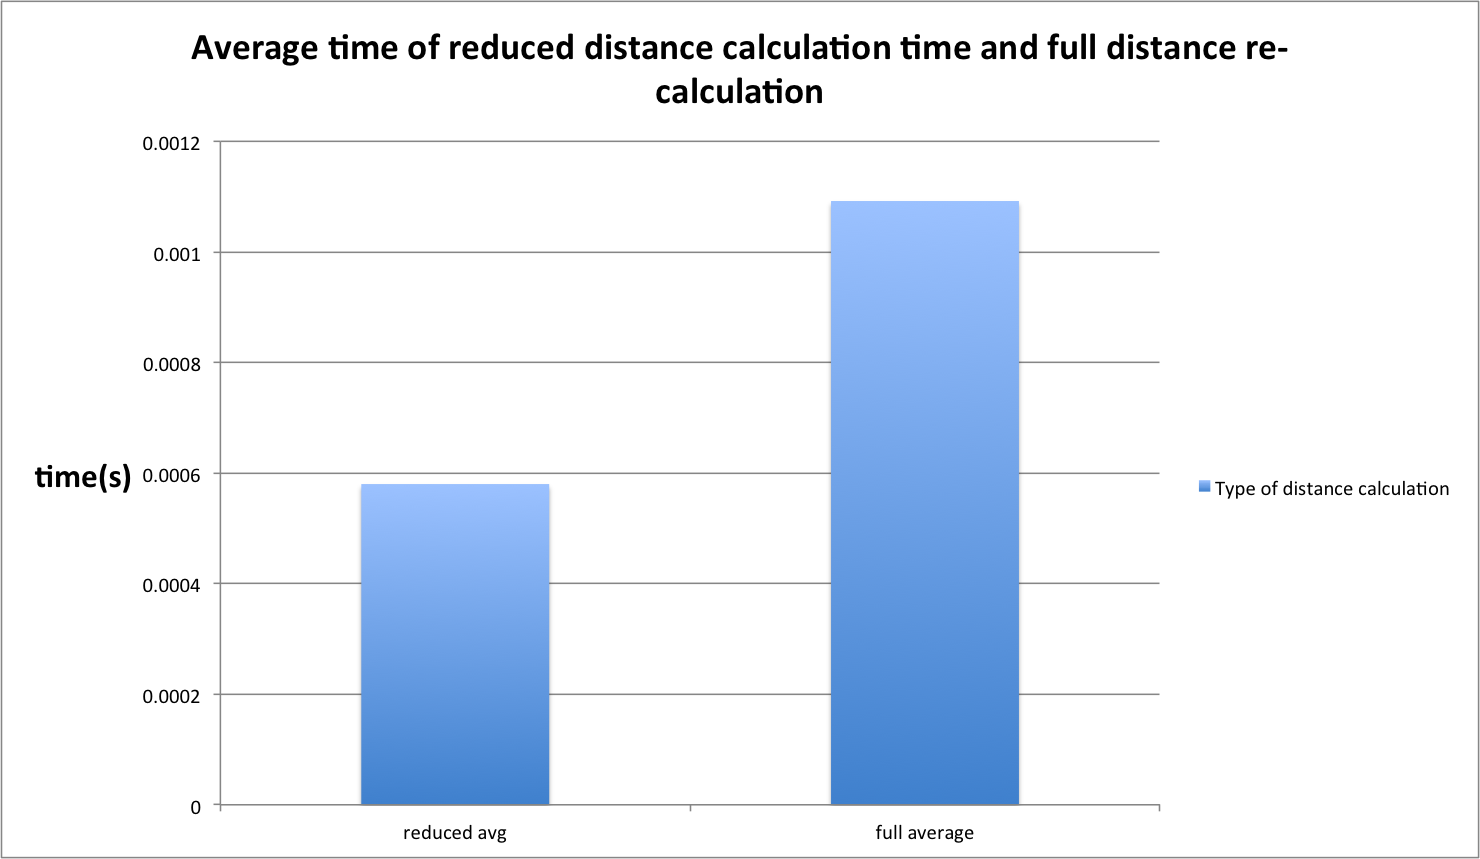
\includegraphics[width=17cm, height=10cm]{../code/misc/reducedvsFullDistanceCalc}
\caption{Average time taken to perform full and partial $\varepsilon$ calculation on the same solution}
\label{f_recalcComparison}
\end{figure}
% talk about how found these values
% talk about testing full against partial by running them and comparing them

\subsection{maxMin and refinedMaxMin}\label{maxMin}
The effect this has on the minimum value that is used in Equation 1, is shown in Figure \ref{f_maxminDif}. The graph shows the minimum scores that are returned by the two methods as green and blue points, as well as the difference between the two values (red line and red numbers) over a single typical competition. From this graph it can be seen that the maxMin method stays relatively low as in this competition the lowest score at the end was only 2 points. On the other hand, the refinedMaxMin method diverges around round 22. This is when it can start ruling out \textit{performers} from winning the overall crown. By the last few round the difference is quite large as there are only a few countries that could still win so only their scores should be taken into account for entertainment.

\begin{figure}[H]
\centering
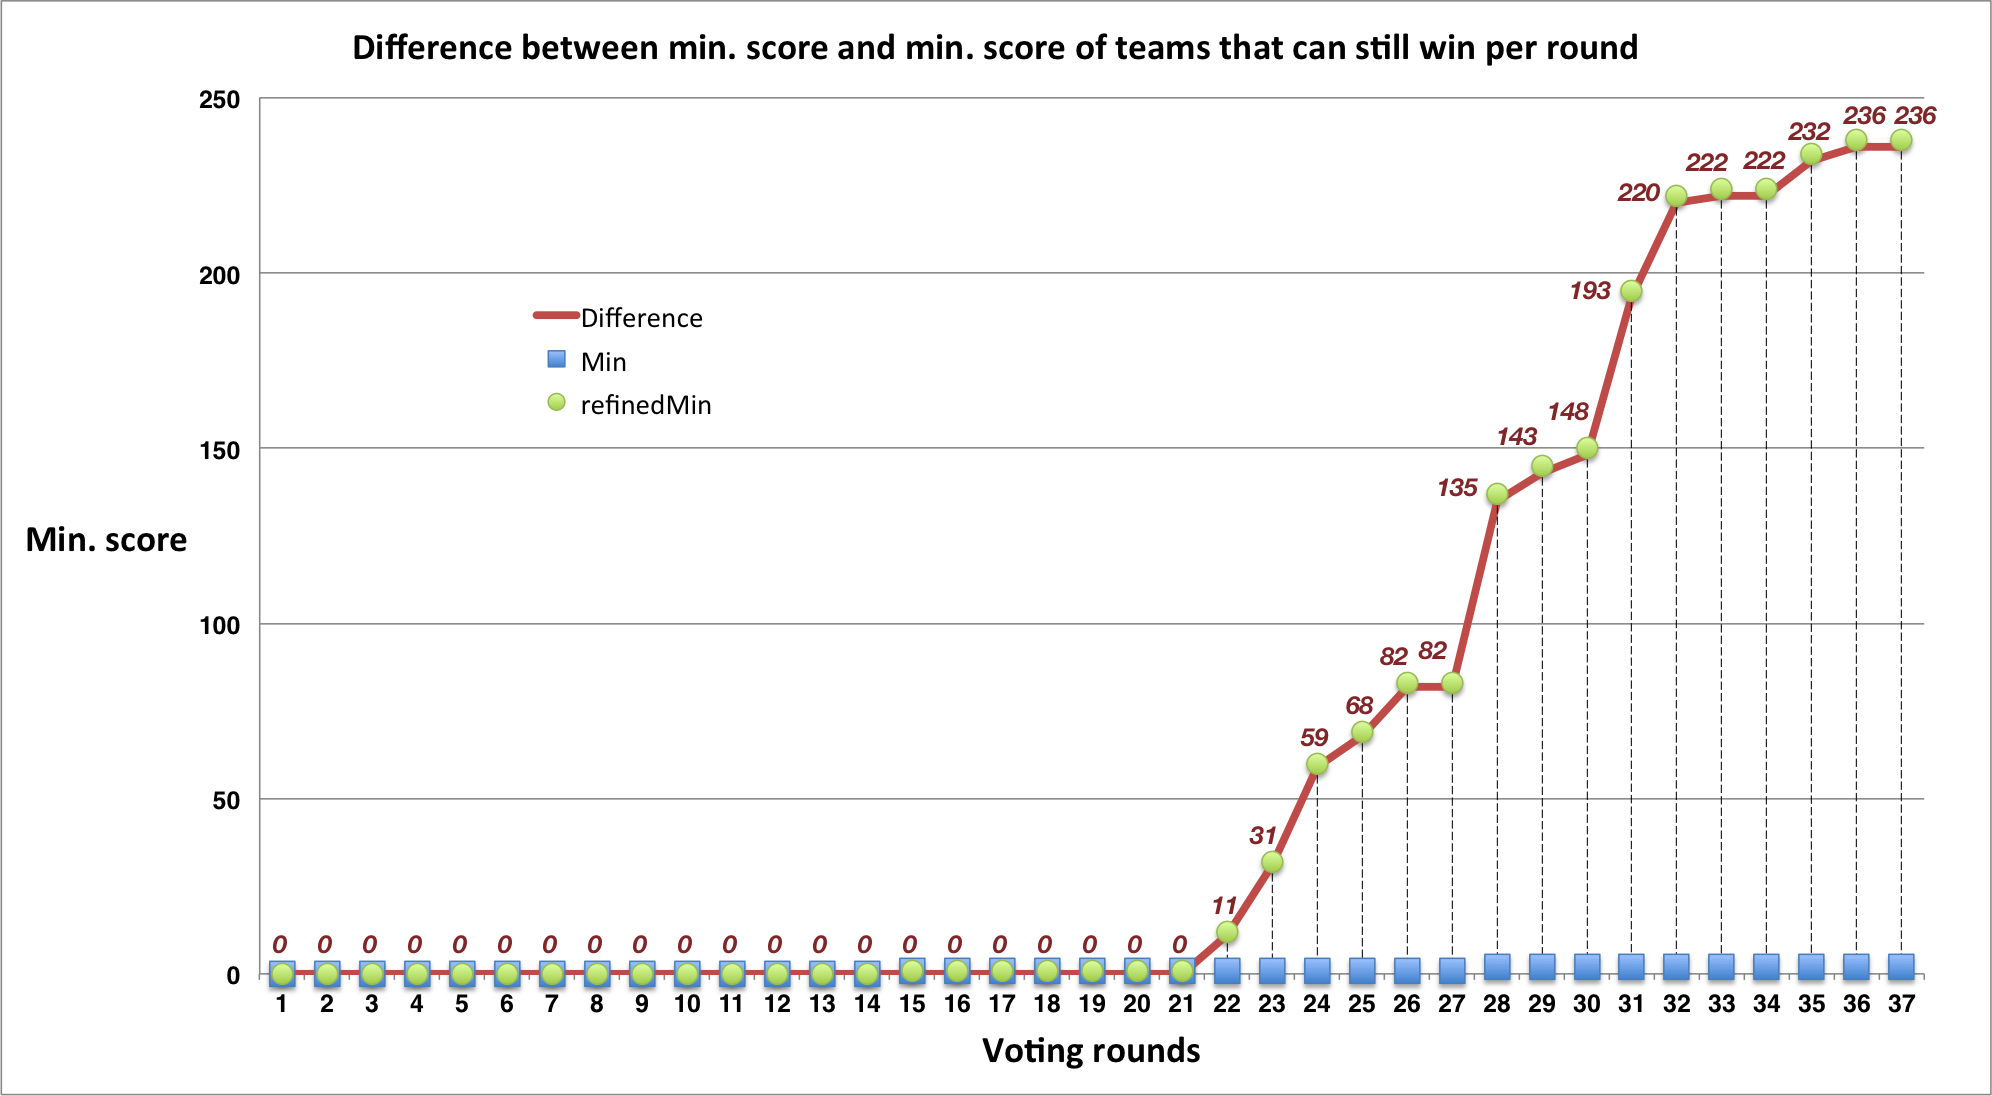
\includegraphics[width=17cm, height=10cm]{../code/misc/difference_MinvsRefinedMin}
\caption{Difference between $min(scores)$ value found for MaxMin method and RefinedMaxMin}
\label{f_maxminDif}
\end{figure}


\subsection{Comparison of Big-O Complexities}
Comparing Simulated Annealing to Greedy Search in equation \ref{greedyCompSimp}, we see that Simulated Annealing and Greedy Search are broadly similar. They are both polynomial time algorithms which when compared to Brute force explains why they can find solutions in a much shorter time. 


\section{Future Work}\label{FutureWork}
% expressing unrealistic ideas, including what you would have liked to have done if only you had not run out of time
% provide a good starting point for someone else to continue the work which you have begun

% is the solution optimal
% evaluating the entertainment function using real world people
% more entertainment functions
% enhance code for performance

\section{Conclusions}\label{Conclusions}
% summary of the aims of the project and a restatement of the main results, i.e. what has been learnt and acheived
% an effective set of conclusions should not introduce new material. Instead it should briefly draw out, summarise, combind and reiterate the main points that have been made in the body of the project report and present opinions based on them

\section{Reflection on Learning}\label{Reflection}
% identify the impact of what we have done on the assumptions, concepts and ideas we used to make decisions about our work
% try to identify the characteristics of the problem that has been addressed , and consider whether assumptions of decisions about the relevant approach to solving the problem had been appropriate, in order to make a better decision in relation to problems that might be encountered in the future.

\section*{Glossary of Terms}
\addcontentsline{toc}{section}{Glossary}
\begin{enumerate}
\item \textbf{Voters ($V$)}: All countries that are in the Eurovision song contest who vote in the final. The voters is a list of countries. It looks like ["Ukraine", "Austria", "France",....]
\item \textbf{Participants ($P$)}: A subset of the voters that perform songs in the final and receive points from the other voters.
\item \textbf{Solution ($\Phi$)}: A solution to the optimisation problem this project is attempting to solve. A solution consists of two things:
	\begin{itemize}
		\item An ordering of the voting countries as a list
		\item An entertainment value found by an entertainment function
	\end{itemize}
\item \textbf{Entertainment Value ($\varepsilon$)}: A value given to a solution that describes how entertaining it is. Calculated using an entertainment function given a solution.
\item \textbf{Round ($R$)}: One round is when one \textit{voter} has given all the \textit{participants} a score. The competition is made up of $n_R$ rounds where $n_R = length of V$.
\item \textbf{Scores ($S$)}: How many points each country has received per round. The scores are an array of the same length as the number of \textit{participants}. It looks like [0,0,2,12,7,4,0,0,3,2,10,....]. When referring to it in the report along with \textbf{rounds} it is most likely cumulative so that after the final round the scores are the total scores for each country.
\end{enumerate}

\section*{Table of Abbreviations}
\addcontentsline{toc}{section}{Table of Abbreviations}

\section*{Appendices}
\addcontentsline{toc}{section}{Appendices}

\begin{table}[H]
\centering
\caption{Big-O complexities of algorithms used}
\label{bigO}
\begin{tabular}{|l|l|}
\hline
        & Big-O time complexity \\ \hline
Greedy Search & $O(V^3)$ \\ \hline
Brute Force & $O(V!)$ \\ \hline
Simulated Annealing & $O(V^4)$ \\ \hline
Piecemeal & $O(V^2)$ \\ \hline
\end{tabular}
\end{table}
All algorithms are expressed in terms of $V$: \textit{voters} and $P$: \textit{participants}. More explanation and calculations can be found in Section \ref{AlgorithmDesigns}.

\clearpage
\renewcommand{\bibsection}{\section*{References}}
\addcontentsline{toc}{section}{References}
\bibliography{./References/finalReportBib}{}
\bibliographystyle{ieeetr}

\end{document}
